\documentclass[12pt]{article}\usepackage[]{graphicx}\usepackage[]{color}
%% maxwidth is the original width if it is less than linewidth
%% otherwise use linewidth (to make sure the graphics do not exceed the margin)
\makeatletter
\def\maxwidth{ %
  \ifdim\Gin@nat@width>\linewidth
    \linewidth
  \else
    \Gin@nat@width
  \fi
}
\makeatother

\definecolor{fgcolor}{rgb}{0.345, 0.345, 0.345}
\newcommand{\hlnum}[1]{\textcolor[rgb]{0.686,0.059,0.569}{#1}}%
\newcommand{\hlstr}[1]{\textcolor[rgb]{0.192,0.494,0.8}{#1}}%
\newcommand{\hlcom}[1]{\textcolor[rgb]{0.678,0.584,0.686}{\textit{#1}}}%
\newcommand{\hlopt}[1]{\textcolor[rgb]{0,0,0}{#1}}%
\newcommand{\hlstd}[1]{\textcolor[rgb]{0.345,0.345,0.345}{#1}}%
\newcommand{\hlkwa}[1]{\textcolor[rgb]{0.161,0.373,0.58}{\textbf{#1}}}%
\newcommand{\hlkwb}[1]{\textcolor[rgb]{0.69,0.353,0.396}{#1}}%
\newcommand{\hlkwc}[1]{\textcolor[rgb]{0.333,0.667,0.333}{#1}}%
\newcommand{\hlkwd}[1]{\textcolor[rgb]{0.737,0.353,0.396}{\textbf{#1}}}%

\usepackage{framed}
\makeatletter
\newenvironment{kframe}{%
 \def\at@end@of@kframe{}%
 \ifinner\ifhmode%
  \def\at@end@of@kframe{\end{minipage}}%
  \begin{minipage}{\columnwidth}%
 \fi\fi%
 \def\FrameCommand##1{\hskip\@totalleftmargin \hskip-\fboxsep
 \colorbox{shadecolor}{##1}\hskip-\fboxsep
     % There is no \\@totalrightmargin, so:
     \hskip-\linewidth \hskip-\@totalleftmargin \hskip\columnwidth}%
 \MakeFramed {\advance\hsize-\width
   \@totalleftmargin\z@ \linewidth\hsize
   \@setminipage}}%
 {\par\unskip\endMakeFramed%
 \at@end@of@kframe}
\makeatother

\definecolor{shadecolor}{rgb}{.97, .97, .97}
\definecolor{messagecolor}{rgb}{0, 0, 0}
\definecolor{warningcolor}{rgb}{1, 0, 1}
\definecolor{errorcolor}{rgb}{1, 0, 0}
\newenvironment{knitrout}{}{} % an empty environment to be redefined in TeX

\usepackage{alltt}

\usepackage{sourcesanspro}
\usepackage{sourcecodepro}
\usepackage{subcaption}

\renewcommand*{\familydefault}{\sfdefault}
\newcommand{\subfloat}[2][need a sub-caption]{\subcaptionbox{#1}{#2}}

\title{Analysis of the {\tt television} data set}
\author{Arthur Allignol}
\date{}




\IfFileExists{upquote.sty}{\usepackage{upquote}}{}
\begin{document}

\maketitle

We read the data using the following command
\begin{knitrout}\scriptsize
\definecolor{shadecolor}{rgb}{0.969, 0.969, 0.969}\color{fgcolor}\begin{kframe}
\begin{alltt}
\hlstd{tele} \hlkwb{<-} \hlkwd{read.csv}\hlstd{(}\hlstr{"/data/Ulm/Teaching/SS_2014/Intro_Biostat_Comp/Illustrations/Television/data/television.csv"}\hlstd{,}
                 \hlkwc{stringsAsFactors} \hlstd{=} \hlnum{FALSE}\hlstd{,} \hlkwc{na.strings} \hlstd{=} \hlstr{"*"}\hlstd{)}
\hlkwd{head}\hlstd{(tele)}
\end{alltt}
\begin{verbatim}
##      Country life    tv phys fem male
## 1  Argentina 70.5   4.0  370  74   67
## 2 Bangladesh 53.5 315.0 6166  53   54
## 3     Brazil 65.0   4.0  684  68   62
## 4     Canada 76.5   1.7  449  80   73
## 5      China 70.0   8.0  643  72   68
## 6   Colombia 71.0   5.6 1551  74   68
\end{verbatim}
\end{kframe}
\end{knitrout}

\noindent 
The aim of the analysis is to assess whether there exists a relation
between the number of people per television set and life
expectancy. 

We first note a couple of facts.
\begin{itemize}
\item Japan is the country with
  the highest life expectancy while
  Ethiopia has the lowest;
\item ``Unsurprisingly'', the United States
  have the lower number of habitants per television set and is equal
  to 1.3.
\end{itemize}
We will first explore the data graphically in
Section~\ref{sec:graph-expl} and perform a simple analysis in
Section~\ref{sec:linear-model}. 

\section{Graphical exploration}\label{sec:graph-expl}

We first display a scatterplot of {\tt life} and {\tt tv} in Figure
\ref{fig:trend_simple}). A trend is clearly to be seen but is
non-linear. 
\begin{knitrout}\scriptsize
\definecolor{shadecolor}{rgb}{0.969, 0.969, 0.969}\color{fgcolor}\begin{kframe}
\begin{alltt}
\hlkwd{ggplot}\hlstd{(tele,} \hlkwd{aes}\hlstd{(}\hlkwc{x} \hlstd{= tv,} \hlkwc{y} \hlstd{= life))} \hlopt{+}
  \hlkwd{geom_jitter}\hlstd{(}\hlkwc{size} \hlstd{=} \hlnum{3}\hlstd{)} \hlopt{+} \hlkwd{geom_smooth}\hlstd{(}\hlkwc{method} \hlstd{=} \hlstr{"lm"}\hlstd{)} \hlopt{+}
  \hlkwd{theme_economist}\hlstd{()}
\end{alltt}


{\ttfamily\noindent\color{warningcolor}{\#\# Warning: Removed 2 rows containing missing values (stat\_smooth).}}

{\ttfamily\noindent\color{warningcolor}{\#\# Warning: Removed 2 rows containing missing values (geom\_point).}}\end{kframe}\begin{figure}[h]

{\centering 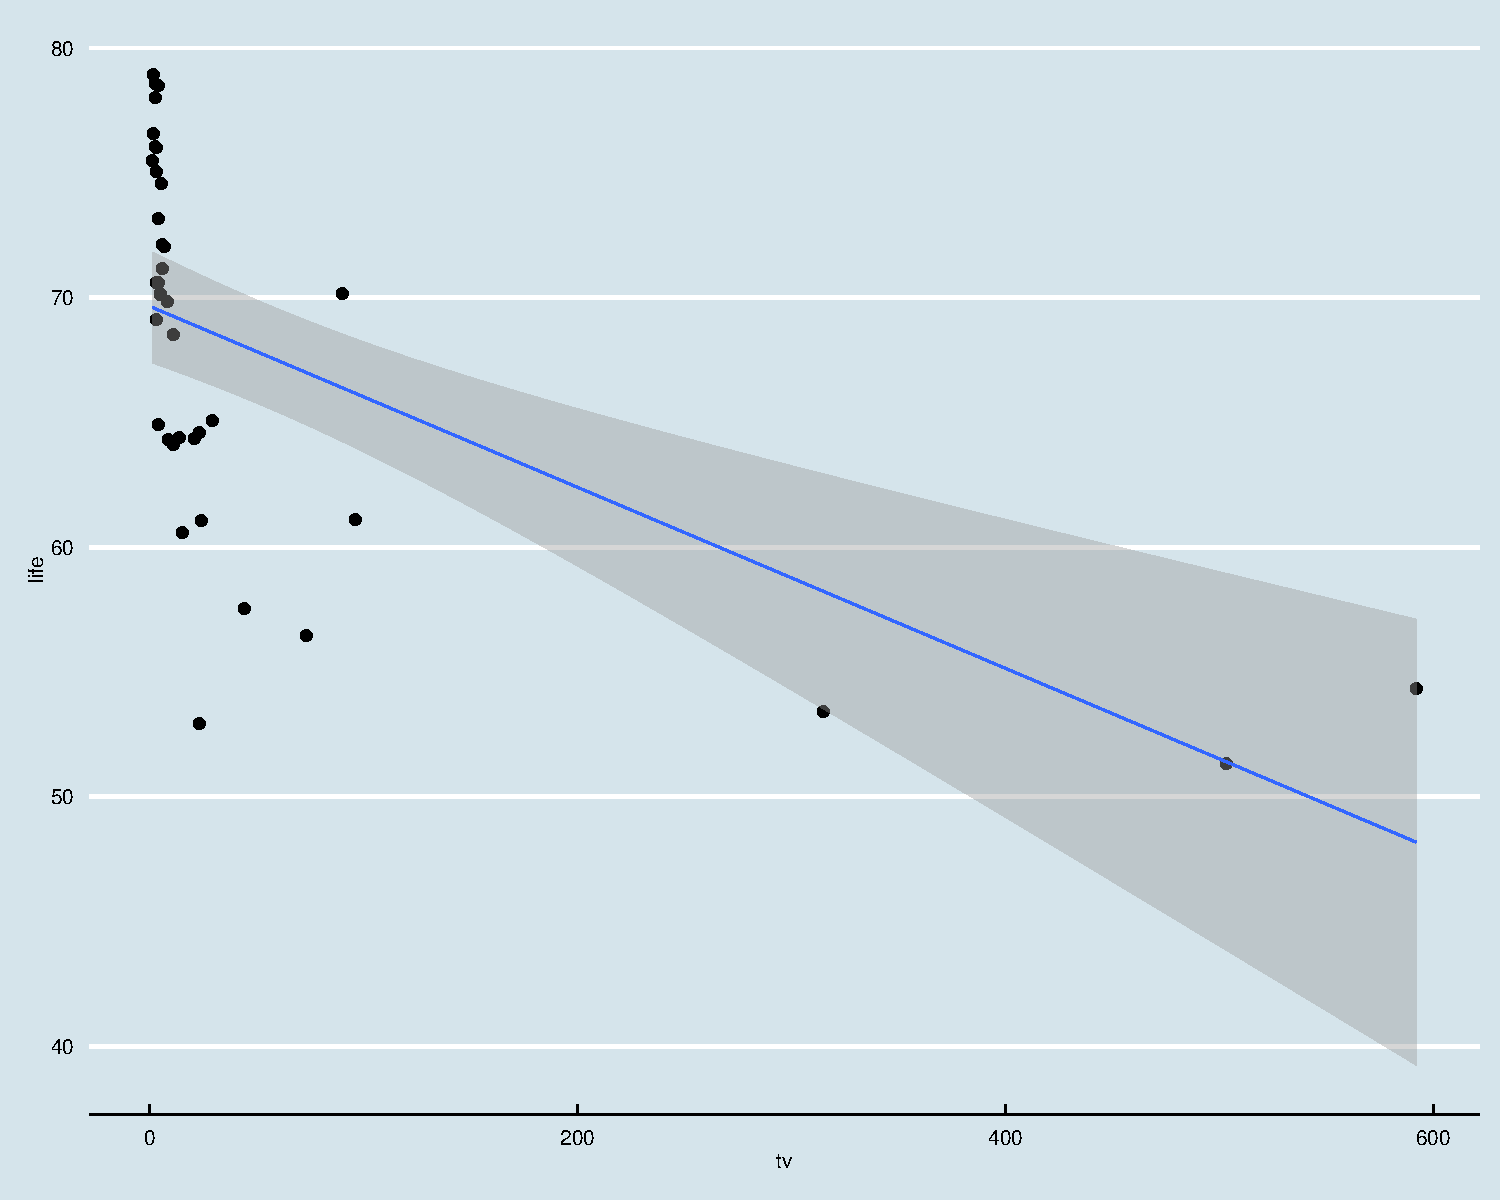
\includegraphics[width=.7\textwidth]{graphics/trend_simple-1} 

}

\caption[Scatterplot of life expectancy and number of individuals per television set]{Scatterplot of life expectancy and number of individuals per television set}\label{fig:trend_simple}
\end{figure}


\end{knitrout}

As a second step, we log-transform the variable {\tt tv}. The relation
between life expectancy and log televisions is in Figure
\ref{fig:log}. The transformation leads to an (almost) perfect linear
relation between these two variables. 
\begin{knitrout}\scriptsize
\definecolor{shadecolor}{rgb}{0.969, 0.969, 0.969}\color{fgcolor}\begin{kframe}
\begin{alltt}
\hlstd{tele}\hlopt{$}\hlstd{log_tv} \hlkwb{<-} \hlkwd{log}\hlstd{(tele}\hlopt{$}\hlstd{tv)}
\hlkwd{ggplot}\hlstd{(tele,} \hlkwd{aes}\hlstd{(}\hlkwc{x} \hlstd{= log_tv,} \hlkwc{y} \hlstd{= life))} \hlopt{+}
  \hlkwd{geom_jitter}\hlstd{(}\hlkwc{size} \hlstd{=} \hlnum{3}\hlstd{)} \hlopt{+} \hlkwd{geom_smooth}\hlstd{(}\hlkwc{method} \hlstd{=} \hlstr{"lm"}\hlstd{)} \hlopt{+}
  \hlkwd{theme_economist}\hlstd{()}
\end{alltt}


{\ttfamily\noindent\color{warningcolor}{\#\# Warning: Removed 2 rows containing missing values (stat\_smooth).}}

{\ttfamily\noindent\color{warningcolor}{\#\# Warning: Removed 2 rows containing missing values (geom\_point).}}\end{kframe}\begin{figure}[h]

{\centering 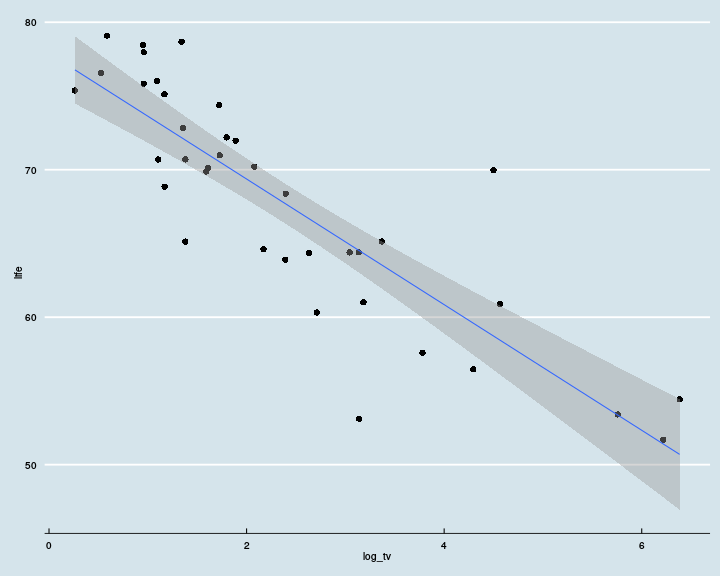
\includegraphics[width=.7\textwidth]{graphics/log-1} 

}

\caption[Scatterplot of life expectancy and log- number of individuals per television set]{Scatterplot of life expectancy and log- number of individuals per television set}\label{fig:log}
\end{figure}


\end{knitrout}


\section{Linear model}\label{sec:linear-model}

We fit a linear model with life expectancy as outcome and the
log-transformed number of individuals per television set.
\begin{knitrout}\scriptsize
\definecolor{shadecolor}{rgb}{0.969, 0.969, 0.969}\color{fgcolor}\begin{kframe}
\begin{alltt}
\hlstd{fit_lm} \hlkwb{<-} \hlkwd{lm}\hlstd{(life} \hlopt{~} \hlkwd{log}\hlstd{(tv), tele)}
\end{alltt}
\end{kframe}
\end{knitrout}
The results are displayed in table \ref{tab:tab_lm}. 
\begin{kframe}
\begin{alltt}
\hlstd{out} \hlkwb{<-} \hlkwd{summary}\hlstd{(fit_lm)}\hlopt{$}\hlstd{coefficients}
\hlstd{out[,} \hlnum{1}\hlopt{:}\hlnum{3}\hlstd{]} \hlkwb{<-} \hlkwd{round}\hlstd{(out[,} \hlnum{1}\hlopt{:}\hlnum{3}\hlstd{],} \hlnum{2}\hlstd{)}
\hlstd{out[,} \hlnum{4}\hlstd{]} \hlkwb{<-} \hlkwd{format.pval}\hlstd{(out[,} \hlnum{4}\hlstd{],} \hlkwc{digits} \hlstd{=} \hlnum{2}\hlstd{,}
                        \hlkwc{eps} \hlstd{=} \hlnum{10}\hlopt{^}\hlstd{(}\hlopt{-}\hlnum{3}\hlstd{))}

\hlkwd{print}\hlstd{(}\hlkwd{xtable}\hlstd{(out,} \hlkwc{caption} \hlstd{=} \hlstr{"Linear model"}\hlstd{,}
             \hlkwc{label} \hlstd{=} \hlstr{"tab:tab_lm"}\hlstd{),}
       \hlkwc{caption.placement} \hlstd{=} \hlstr{"top"}\hlstd{)}
\end{alltt}
\end{kframe}% latex table generated in R 3.2.0 by xtable 1.7-4 package
% Wed Apr 29 23:49:41 2015
\begin{table}[ht]
\centering
\caption{Linear model} 
\label{tab:tab_lm}
\begin{tabular}{rllll}
  \hline
 & Estimate & Std. Error & t value & Pr($>$$|$t$|$) \\ 
  \hline
(Intercept) & 77.89 & 1.22 & 63.83 & $<$0.001 \\ 
  log(tv) & -4.26 & 0.43 & -9.9 & $<$0.001 \\ 
   \hline
\end{tabular}
\end{table}

We can check the model fit by plotting the residuals versus the fitted
values (Figure \ref{fig:res_vs_fit}).
\begin{knitrout}\scriptsize
\definecolor{shadecolor}{rgb}{0.969, 0.969, 0.969}\color{fgcolor}\begin{kframe}
\begin{alltt}
\hlstd{df} \hlkwb{<-} \hlkwd{fortify}\hlstd{(fit_lm)}
\hlkwd{ggplot}\hlstd{(df,} \hlkwd{aes}\hlstd{(.fitted, .resid))} \hlopt{+}
  \hlkwd{geom_point}\hlstd{(}\hlkwc{size} \hlstd{=} \hlnum{2}\hlstd{)}  \hlopt{+}
  \hlkwd{geom_smooth}\hlstd{(}\hlkwc{se}\hlstd{=}\hlnum{FALSE}\hlstd{)} \hlopt{+}
  \hlkwd{scale_x_continuous}\hlstd{(}\hlstr{"Fitted Values"}\hlstd{)} \hlopt{+}
  \hlkwd{scale_y_continuous}\hlstd{(}\hlstr{"Residual"}\hlstd{)} \hlopt{+}
  \hlkwd{labs}\hlstd{(}\hlkwc{title} \hlstd{=} \hlstr{"Residuals vs fitted"}\hlstd{)} \hlopt{+}
  \hlkwd{theme_economist}\hlstd{()}
\end{alltt}


{\ttfamily\noindent\itshape\color{messagecolor}{\#\# geom\_smooth: method="{}auto"{} and size of largest group is <1000, so using loess. Use 'method = x' to change the smoothing method.}}\end{kframe}\begin{figure}[h]

{\centering 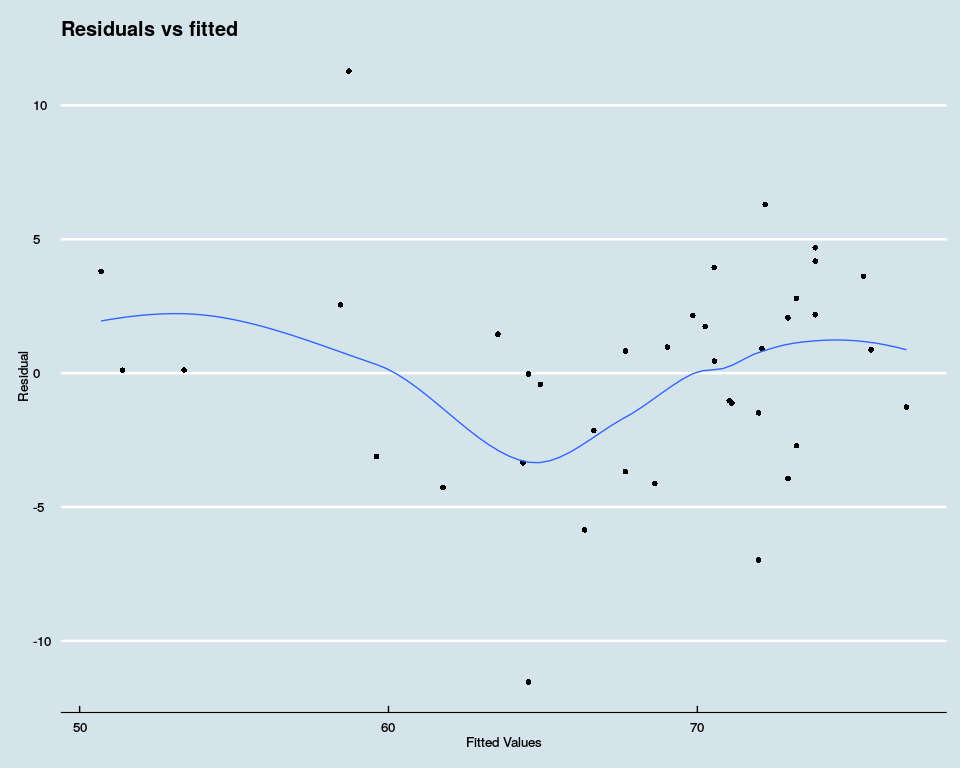
\includegraphics[width=.7\textwidth]{graphics/res_vs_fit-1} 

}

\caption[Residuals VS fitted]{Residuals VS fitted}\label{fig:res_vs_fit}
\end{figure}


\end{knitrout}



\end{document}
